\documentclass[a4paper,12pt]{extarticle}
\usepackage[utf8x]{inputenc}
\usepackage[T1,T2A]{fontenc}
\usepackage[russian]{babel}
\usepackage{hyperref}
\usepackage{indentfirst}
\usepackage{listings}
\usepackage{color}
\usepackage{here}
\usepackage{array}
\usepackage{multirow}
\usepackage{graphicx}
\usepackage{amsmath}
\usepackage{amssymb}

\usepackage{caption}
\renewcommand{\lstlistingname}{Программа} % заголовок листингов кода

\bibliographystyle{ugost2008ls}

\usepackage{listings}
\lstset{ %
extendedchars=\true,
keepspaces=true,
language=C,						% choose the language of the code
basicstyle=\footnotesize,		% the size of the fonts that are used for the code
numbers=left,					% where to put the line-numbers
numberstyle=\footnotesize,		% the size of the fonts that are used for the line-numbers
stepnumber=1,					% the step between two line-numbers. If it is 1 each line will be numbered
numbersep=5pt,					% how far the line-numbers are from the code
backgroundcolor=\color{white},	% choose the background color. You must add \usepackage{color}
showspaces=false				% show spaces adding particular underscores
showstringspaces=false,			% underline spaces within strings
showtabs=false,					% show tabs within strings adding particular underscores
frame=single,           		% adds a frame around the code
tabsize=2,						% sets default tabsize to 2 spaces
captionpos=t,					% sets the caption-position to top
breaklines=true,				% sets automatic line breaking
breakatwhitespace=false,		% sets if automatic breaks should only happen at whitespace
escapeinside={\%*}{*)},			% if you want to add a comment within your code
postbreak=\raisebox{0ex}[0ex][0ex]{\ensuremath{\color{red}\hookrightarrow\space}},
texcl=true,
inputpath=listings,                     % директория с листингами
}

\usepackage[left=2cm,right=2cm,
top=2cm,bottom=2cm,bindingoffset=0cm]{geometry}

%% Нумерация картинок по секциям
\usepackage{chngcntr}
\counterwithin{figure}{subsection}
\counterwithin{table}{section}

%%Точки нумерации заголовков
\usepackage{titlesec}
\titlelabel{\thetitle.\quad}
\usepackage[dotinlabels]{titletoc}

%% Оформления подписи рисунка
\addto\captionsrussian{\renewcommand{\figurename}{Рис.}}
\captionsetup[figure]{labelsep = period}

%% Подпись таблицы
\DeclareCaptionFormat{hfillstart}{\hfill#1#2#3\par}
\captionsetup[table]{format=hfillstart,labelsep=newline,justification=centering,skip=-10pt,textfont=bf}

%% Путь к каталогу с рисунками
\graphicspath{{fig/}}

\begin{document}	% начало документа
\setcounter{tocdepth}{3}

% Титульная страница
\begin{titlepage}	% начало титульной страницы

	\begin{center}		% выравнивание по центру

		\large Санкт-Петербургский Политехнический Университет Петра Великого\\
		\large Институт компьютерных наук и технологий \\
		\large Кафедра компьютерных систем и программных технологий\\[6cm]
		% название института, затем отступ 6см
		
		\huge Телекоммуникационные технологии\\[0.5cm] % название работы, затем отступ 0,5см
		\large Отчет по лабораторной работе №3\\[0.1cm]
		\large Линейная фильтрация\\[5cm]

	\end{center}


	\begin{flushright} % выравнивание по правому краю
		\begin{minipage}{0.25\textwidth} % врезка в половину ширины текста
			\begin{flushleft} % выровнять её содержимое по левому краю

				\large\textbf{Работу выполнил:}\\
				\large Беседин Д.С.\\
				\large {Группа:} 33501/3\\
				
				\large \textbf{Преподаватель:}\\
				\large Богач Н.В.

			\end{flushleft}
		\end{minipage}
	\end{flushright}
	
	\vfill % заполнить всё доступное ниже пространство

	\begin{center}
	\large Санкт-Петербург\\
	\large \the\year % вывести дату
	\end{center} % закончить выравнивание по центру

\thispagestyle{empty} % не нумеровать страницу
\end{titlepage} % конец титульной страницы

\vfill % заполнить всё доступное ниже пространство

% Содержание
% Содержание
\renewcommand\contentsname{\centerline{Содержание}}
\tableofcontents
\newpage


\section{Цель и задачи}

\subsection{Цель работы}
Изучение методов помехоустойчивого кодирования и сравнения их свойств.
 
\subsection{Постановка задачи}
Провести кодирование/декодирование сигнала, полученного с помощью функции randerr кодом Хэмминга 2-мя способами: с помощью встроенных функций encode/decode, а также через создание проверочной и генераторной матриц и вычисление синдрома. Оценить корректирующую способность кода.

Выполнить кодирование/декодирование циклическим кодом, кодом БЧХ, кодом Рида-Соломона. Оценить корректирующую способность кода.

 
\section{Теоретическая информация}

\subsection{Кодирование}
Физическое кодирование — линейное преобразование двоичных данных, осуществляемое для их передачи по физическому каналу. Физическое кодирование может менять форму, ширину полосы частот и гармонический состав сигнала в целях осуществления синхронизации приёмника и передатчика, устранения постоянной составляющей или уменьшения аппаратных затрат передачи сигнала.

Обнаружение ошибок в технике связи — действие, направленное на контроль целостности данных при записи/воспроизведении информации или при её передаче по линиям связи. Исправление ошибок (коррекция ошибок) — процедура восстановления информации после чтения её из устройства хранения или канала связи.

Для обнаружения ошибок используют коды обнаружения ошибок, для исправления — корректирующие коды (коды, исправляющие ошибки, коды с коррекцией ошибок, помехоустойчивые коды).

\subsection{Типы помехоустойчивого кодирования}
\subsubsection{Кодирование Хэмминга}
Коды Хемминга — простейшие линейные коды с минимальным расстоянием 3, то есть способные исправить одну ошибку. Код Хемминга может быть представлен в таком виде, что синдром
\begin{equation}
\vec{s} = \vec{r} H^T
\end{equation}

Этот принятый вектор будет равен номеру позиции, в которой произошла ошибка. Это свойство позволяет сделать декодирование очень простым.

Коды, в которых возможно автоматическое исправление ошибок, называются самокорректирующимися. Коды Хэмминга являются самоконтролирующимися кодами, то есть кодами, позволяющими автоматически обнаруживать ошибки при передаче данных и исправлять их.

Для построения самокорректирующегося кода, рассчитанного на исправление одиночных ошибок, одного контрольного разряда недостаточно. Как видно из дальнейшего, количество контрольных разрядов k должно быть выбрано так, чтобы удовлетворялось неравенство 
\begin{equation}
2^{k}\geq k+m+1
\end{equation}
или  
\begin{equation}
k \geq \log _{2}(k+m+1) 
\end{equation}
где m — количество основных двоичных разрядов кодового слова.

Минимальные значения k при заданных значениях m, найденные в соответствии с этим неравенством, приведены в таблице.
\begin{figure}[H]
	\begin{center}
		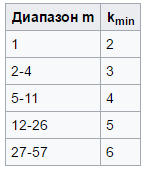
\includegraphics[width=0.2\linewidth]{Table_kmin.png}
		\caption{Значения $K_{min}$ в зависимости от $m$} %% подпись к рисунку
		\label{Table_kmin} %% метка рисунка для ссылки на него
	\end{center}
\end{figure}

Построение кодов Хэмминга основано на принципе проверки на четность числа единичных символов: к последовательности добавляется такой элемент, чтобы число единичных символов в получившейся последовательности было четным.

\begin{equation}
	r_1 = i_1 \oplus i_2 \oplus ... \oplus i_k
\end{equation}

\begin{equation}
	S = i_1 \oplus i_2 \oplus ... \oplus i_n \oplus r_1
\end{equation}
Тогда если $S = 0$ - ошибки нет, иначе есть однократная ошибка.

Такой код называется $(k+1,k)$. Первое число — количество элементов последовательности, второе — количество информационных символов.

Получение кодового слова выглядит следующим образом:
\begin{equation}
( i_1 \> i_2 \> i_3 \> i_4 )  \begin{pmatrix}
1 & 0 & 0 & 0 & 1 & 0 & 1 \\
0 & 1 & 0 & 0 & 1 & 1 & 1 \\         
0 & 0 & 1 & 0 & 1 & 1 & 0 \\
0 & 0 & 0 & 1 & 0 & 1 & 1
\end{pmatrix} = ( i_1 \> i_2 \> i_3 \> i_4  \> r_1  \> r_2  \> r_3)
\end{equation}

Получение синдрома выглядит следующим образом:

\begin{equation}
(i_{1} \> i_{2} \> i_{3} \> i_{4} \> r_{1} \> r_{2} \> r_{3} )  \begin{pmatrix}
1 & 0 & 1 \\
1 & 1 & 1 \\
1 & 1 & 0 \\
0 & 1 & 1 \\
1 & 0 & 0 \\
0 & 1 & 0 \\
0 & 0 & 1 \\ 
\end{pmatrix} = \begin{pmatrix}S_{1}&S_{2}&S_{3}\\\end{pmatrix}
\end{equation}

\subsubsection{Циклические коды}
Циклический код — линейный код, обладающий свойством цикличности, то есть каждая циклическая перестановка кодового слова также является кодовым словом. Используется для преобразования информации для защиты её от ошибок.

\subsubsection{Коды БЧХ}
Коды Боуза — Чоудхури — Хоквингема (БЧХ-коды) — в теории кодирования это широкий класс циклических кодов, применяемых для защиты информации от ошибок. Отличается возможностью построения кода с заранее определёнными корректирующими свойствами, а именно, минимальным кодовым расстоянием. Частным случаем БЧХ-кодов является код Рида — Соломона.

\subsubsection{Коды Рида-Соломона}
Коды Рида—Соломона (англ. Reed–Solomon codes) — недвоичные циклические коды, позволяющие исправлять ошибки в блоках данных. Элементами кодового вектора являются не биты, а группы битов (блоки).
Код Рида—Соломона является частным случаем БЧХ-кода.

\section{Ход работы}

Реализация различных типов кодирования с помощью MATLAB:
\lstinputlisting[
	label=code:code,
	caption={Код в МатЛаб},% для печати символ '_' требует выходной символ '\'
]{Code.m}

\subsection{Коды Хэмминга}
Ниже представлены сообщение и его код, полученный стандартной функцией encode с параметром 'hamming/binary' (использовался стандартный код Хемминга (7,4)).
\begin{figure}[H]
	\begin{center}
		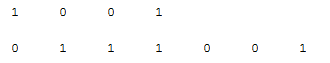
\includegraphics[width=1\linewidth]{Ham_Code.png}
		\caption{Исходное сообщение и его код Хэмминга} %% подпись к рисунку
		\label{Ham_Code} %% метка рисунка для ссылки на него
	\end{center}
\end{figure}
При кодировании сообщений с кодовым расстоянием, равным 1, получали, как пример, закодированные сообщения с кодовым расстоянием равным 3.

\subsection{Циклические коды}
Ниже представлено сообщение, закодированное циклическим кодом, полученным стандартной функцией encode с параметром 'cyclic/binary' (использовался стандартный код (7,4)).
\begin{figure}[H]
	\begin{center}
		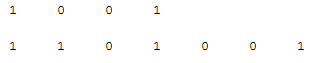
\includegraphics[width=1\linewidth]{Cyclic_Code.png}
		\caption{Исходное сообщение и его циклический код} %% подпись к рисунку
		\label{Cyclic_Code} %% метка рисунка для ссылки на него
	\end{center}
\end{figure}
При кодировании сообщений с кодовым расстоянием, равным 1, получали, как пример, закодированные сообщения с кодовым расстоянием равным 3.

\subsection{Коды БЧХ}
Для кодирования/декодирования с помощью кодов БЧХ использовались, соответственно, функции bchenc/bchdec.
При кодировании сообщений с кодовым расстоянием, равным 1, получали, как пример, закодированные сообщения с кодовым расстоянием равным 3, или 4.
Массивы до и после декодирования представлены на Рис.\ref{Bch_code} и Рис.\ref{Bch_decode}:
\begin{figure}[H]
	\begin{center}
		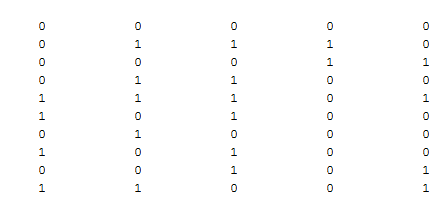
\includegraphics[width=1\linewidth]{Bch_code.png}
		\caption{Масисв до декодирования} %% подпись к рисунку
		\label{Bch_code} %% метка рисунка для ссылки на него
	\end{center}
\end{figure}
\begin{figure}[H]
	\begin{center}
		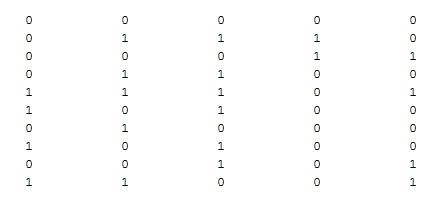
\includegraphics[width=1\linewidth]{Bch_decode.png}
		\caption{Массив после декодирования} %% подпись к рисунку
		\label{Bch_decode} %% метка рисунка для ссылки на него
	\end{center}
\end{figure}

\subsection{Коды Рида-Соломона}
При использовании кодов Рида-Соломона в виде стандартной функции rsenc можно наблюдать вектор cnumerr, который содержит количества исправляемых ошибок.
\begin{figure}[H]
	\begin{center}
		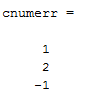
\includegraphics[width=0.2\linewidth]{cnumerr.png}
		\caption{Количество исправляемых ошибок cnumerr} %% подпись к рисунку
		\label{cnumerr} %% метка рисунка для ссылки на него
	\end{center}
\end{figure}
При кодировании сообщений с кодовым расстоянием, равным 1, получали, как пример, закодированные сообщения с кодовым расстоянием равным 3, или 4.

\section{Выводы}
Кодирование - важный процесс при передаче сигналов по каналам связи. Методы кодирования дополняют методы модуляции для обеспечения улучшения качества передачи, для предотвращения ошибок при передаче, а также защищенности данных от получения злоумышлинниками.
Рассмотрены различные методы кодирования - коды Хэмминга, циклические коды, коды БЧХ, коды Рида-Соломона, которые являются самокорректирующимися, т.е. могу исправлять ошибки, полученные из-за влияния помех на сигнал в процессе передачи.

\end{document}
